% Copyright Aidan Randle-Conde 2007-2014
% http://www.aidansean.com/phd_notes
% Anyone is free to download, redistribute, edit and use these notes and the source tex files with the following restrictions:
% This 
%  This message is included in the tex source files.
%  Aidan Randle-Conde is credited as the author.
%  Images are correctly credited to their respective authors, as outlined in the references.
%  No part of these notes may be used for commercial purposes.

\chapter{Neutral current interactions}

\section{Weinberg-Salam model}

The Weinberg-Salam model makes it possible to find the neutral current (NC) couping to the $Z^0$ to the fundamental particles.  The couplings described here survive symmetry breaking.  A certain structure was perceived in the charged current weak process and certain similarities were seen between the weak interaction and the electromagnetic interaction.

The charged current weak interaction operates between left-handed lepton and quark doublets (the quark doublets are modified by the CKM matrix).

The left-handed doublets are:

\[
  \chi_L = \frac{1}{2}\left(1 - \gamma^5\right)
  \left(
  \begin{array}{c}
    \nu_l \\
    l^-
  \end{array}
  \right)
\]

and when a $W^+$ is absorbed (as shown in figure \ref{fig:ch13_WENu}) the matrix element is:

\begin{figure}[!htb]
  \begin{center}
    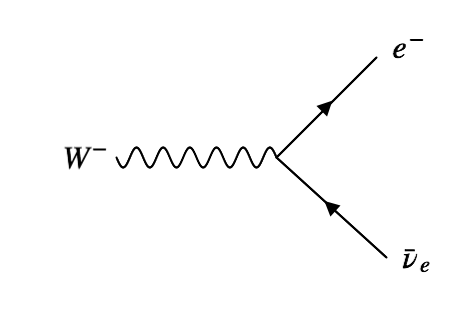
\includegraphics[width=0.4\textwidth]{images/web_feynman/image_56.png}
    \caption[Decay of $W\to e\nu_e$]{Decay of $W\to e\nu_e$.}
    \label{fig:ch13_WENu}
  \end{center}
\end{figure}

\begin{eqnarray*}
  \bar{u}_{\nu}\gamma^{\mu}\frac{1}{2}\left(1 - \gamma^5\right)u_{\e} & = & \bar{u}_{\nu}\gamma^{\mu}\left(\frac{1}{2}\right)^2\left(1 - \gamma^5\right)^2u_{\e} \\
  & = & \bar{u}_{\nu}\frac{1}{2}\left(1 + \gamma^5\right)\gamma^{\mu}\frac{1}{2}\left(1 - \gamma^5\right)u_{\e}
\end{eqnarray*}

Using the two component weak iso-spinors it can be written:

\[
  \bar{\chi}_L \gamma^{\mu}\tau^+\chi_L
\]

where $\tau$ is the raising operator in weak isospin space (with ordinary spin, $\sigma^+$ is used rather than $\tau^+$).

The electromagnetic current is:

\begin{eqnarray*}
  j^{\mu}_{em} & = & -\e \bar{u}\gamma^{\mu}\e \\
  \textrm{or } j^{\mu}_{em} & = & -\e\left(\bar{u}_L\gamma^{\mu}u_L + \bar{u}_R\gamma^{\mu}r_R\right)
\end{eqnarray*}

Going back to the charged current interaction:

\begin{eqnarray*}
  \tau^+ & = & \frac{\tau_x + i\tau_y}{2} \\
  & = &
  \left(
  \begin{array}{cc}
    0 & 1 \\
    0 & 0
  \end{array}
  \right)
  \\
  \bar{\chi}_L\gamma^{\mu}\tau^+\chi_L & = & \left(\bar{\nu}_{\e}\bar{\e}^-\right)_L\gamma^{\mu}
  \left(
  \begin{array}{cc}
    0 & 1 \\
    0 & 0
  \end{array}
  \right)
  \left(
  \begin{array}{c}
    \nu_{\e} \\
    \e^-
  \end{array}
  \right)_L \\
  & = & \bar{\nu}_{\e}\gamma^{\mu}\e^-_L
\end{eqnarray*}

If the symmetry were exact then the following interaction would be expected:

\begin{eqnarray*}
  \left( \bar{\nu}_{\e} \quad \bar{\e}^-\right)_L \gamma^{\mu}\frac{1}{2}
  \left(
    \begin{array}{cc}
      1 & 0 \\
      0 & -1
    \end{array}
    \right)
    \left(
    \begin{array}{c}
      \nu_{\e} \\
      \e^-
    \end{array}
    \right)_L
    = \frac{1}{2}\bar{\nu}\gamma^{\mu}\nu - \frac{1}{2}\bar{\e}^-_L\gamma^{\mu}\e^-_L
\end{eqnarray*}

However this neutral current does not exist.  This theory was proposed before the discovery of neutral currents.  When it was observed, it was not compatible with the above form.

There was another entity which is the right-handed electron.  Since this object is not involved in charged current weak interactions it must be a singlet in weak isospin space.  So a new quantity must be invented which differentiates between the states in the $\left( \begin{array}{cc}\nu_{\e}\\\e^-\end{array}\right)_L$ doublet and the singlet $\left(\e^-\right)_R$ ie the members of the doublet must have the same value of this new quantum number.

This quantum numbers is the weak hypercharge:

\[
  Y = 2Q - 2I^3
\]

For some typical particles:

\[
  \begin{array}{c|c|c|c}
             & I_3  & Q    & Y    \\
    \hline
    \nu_{\e} & 1/2  & 0    & -1   \\
    \e^-_L   & -1/2 & -1   & -1   \\
    \e^-_R   & 0    & -1   & -2   \\
    u_L      & 1/2  & 2/3  & -1/3 \\
    d_L      & -1/2 & -1/3 & 1/3  \\
    u_R      & 0    & 2/3  & 4/3  \\
    d_R      & 0    & -1/3 & -2/3
  \end{array}
\]

In the internal space of electroweak interactions the hypercharge resembles ordinary charge.

For the electromagnetic interaction the wavefunctions can be multiplied by phase factors ie $\psi' = \e^{iq\chi}\psi$.  If $\chi$ is just a number such a transformation is called a global gauge transformation.  However if $\chi = \chi(\ul{r},t)$ then there is a local gauge transformation and the electromagnetic field $A^{\mu}$ had to be introduced so that the gauge invariance of the Lagrangian (or equations of motion, eg Dirac equation) is preserved.

If the new theory is required to be invariant with respect to local gauge transformations, and is of the form:

\[
  \e^{iY\chi(\ul{r},t)} \quad Y = \textrm{hypercharge}
\]

then a massless $B^{\mu}$ field has to be introduced.

The weak left-handed isospinor is transformed by a (special) unitary transformation involving $3$ parameters.  Alternatively the $SU(2)$ spinor is in an $O(3)$ space which requires $3$ axes.  These axes can be defined locally under a gauge transformation and $3$ weak massless fields must be introduced if the system is to be invariant with respect to these local gaue transformations.

The fields are going to interact with the currents in the theory.  These fields also interact with themselves which gives rise to the trilinear and quadrilinear couplings.

The interaction will be of the form:

\begin{eqnarray*}
  && g_W\bar{\chi}_L\gamma^{\mu}\frac{\tau^i}{2}\chi_L W^i_{\mu} + \frac{g'}{2}j^Y_{\mu}B^{\mu} \\
  & \textrm{or } & g_W\bar{\chi}_L\gamma^{\mu}\frac{\tau^i}{2}\chi_L W^i_{\mu} + g'\left(j^{em}_{\mu} - j^{I^3}_{\mu}\right)B^{\mu}
\end{eqnarray*}

So the electromagnetic current is a combination of the hypercharge and isospin.

Considering the first term on the left, when the symmetry breaks, the massless $W^1$ and $W^2$ fields combine to give massive $W^+$ and $W^-$ vector bosons.  When symmetry breaking occurs the $W^3_{\mu}$ and $B_{\mu}$ fields mix to give a massless photon, $A_{\mu}$, and the massive $Z^0_{\mu}$.

\begin{eqnarray*}
  \textrm{ie } &
  \left(
  \begin{array}{c}
    A_{\mu} \\
    Z^0_{\mu}
  \end{array}
  \right)
  & =
  \left(
  \begin{array}{cc}
     \cos\theta_W & \sin\theta_W \\
    -\sin\theta_W & \cos\theta_W
  \end{array}
  \right)
  \left(
  \begin{array}{c}
    B_{\mu} \\
    W^3_{\mu}
  \end{array}
  \right)
  \\
  \textrm{or } &
  \left(
  \begin{array}{c}
    B_{\mu} \\
    W^3_{\mu}
  \end{array}
  \right)
  & =
  \left(
  \begin{array}{cc}
    \cos\theta_W & -\sin\theta_W \\
    \sin\theta_W &  \cos\theta_W
  \end{array}
  \right)
  \left(
  \begin{array}{c}
    A_{\mu} \\
    Z^0_{\mu}
  \end{array}
  \right)
\end{eqnarray*}

$\theta_W$ is the Weinberg, or weak, mixing angle.

$g_W j^3_{\mu} W^{\mu}_3 + g'\left(j^{\mu}_{em} - j^{\mu}_3\right)B_{\mu}$ can be expressed in terms of $A_{\mu}$ and $Z^0_{\mu}$:

\begin{eqnarray*}
  \textrm{using } & B_{\mu}   & = A_{\mu}\cos\theta_W - Z^0_{\mu}\sin\theta_W \\
  \textrm{and }   & W^3_{\mu} & = A_{\mu}\sin\theta_W + Z^0_{\mu}\cos\theta_W
\end{eqnarray*}

\begin{eqnarray*}
  g_W j^3_{\mu} W^{\mu}_3 + g'\left(j^{\mu}_{em} - j^{\mu}_3\right)B_{\mu} & = & \left(g_W j^3_{\mu} \sin\theta_W + g'j^{em}_{\mu}\cos\theta_W - g'j^3_{\mu}\cos\theta_W\right)A^{\mu} \\
  & & + \left(g_W j^3_{\mu} \cos\theta_W - g'j^{em}_{\mu}\sin\theta_W + g'j^3_{\mu}\sin\theta_W\right)Z^0
\end{eqnarray*}

But the $A^{\mu}$ field couples only to the electromagnetic interaction so the first and third terms sum to zero:

\begin{eqnarray*}
  \Rightarrow g_W j^3_{\mu}\sin\theta_W & = & g' j^3_{\mu}\cos\theta_W \\
  \Rightarrow g' & = & g_W \tan\theta_W
\end{eqnarray*}

and from the second term:

\begin{eqnarray*}
  g_W\tan\theta_W\cos\theta_W & = & \e \\
  \Rightarrow g_W\sin\theta_W & = & \e \\
  \textrm{or } g'\cos\theta_W & = & \e
\end{eqnarray*}

So the two couplings $g_W$ and $g'$ can be replaced by $\e$ and $\theta_W$ where $\theta_W$ is determined by experiment.

From the $Z^0_{\mu}$ terms it is possible to get the coupling of the $Z^0$ to the leptons and quarks.

\[
  \Big[g_Wj^3_{\mu}\cos\theta_W - g_W\tan\theta_Wj^{em}_{\mu}\sin\theta_W + g_W\tan\theta_W j^3_{\mu}\sin\theta_W\Big] Z^{\mu}
\]

\begin{eqnarray*}
  & = & \Bigg[ g_Wj^3_{\mu}\cos\theta_W - g_W\frac{\sin^2\theta_W}{\cos\theta_W}j^{em}_{\mu} + g_W\frac{\sin^2\theta_W}{\cos\theta_W}j^3_{\mu}\Bigg]Z^{\mu} \\
  & = & \frac{g_W}{\cos\theta_W}\Big[j^3_{\mu}\cos^2\theta_W - j^{em}_{\mu}\sin^2\theta_W + j^3_{\mu}\sin^2\theta_W\Big]Z^{\mu} \\
  & = & \frac{g_W}{\cos\theta_W}\Big[j^3_{\mu} - j^{em}_{\mu}\sin^2\theta_W\Big]Z^{\mu} \\
  \Rightarrow j^{NC}_{\mu} & = & j^3_{\mu} - j^{em}_{\mu}\sin^2\theta_W
\end{eqnarray*}

Inserting the forms of the currents gives:

\begin{eqnarray*}
  j^{NC}_{\mu} & = & \bar{\psi}_f \gamma^{\mu}\left( \frac{1}{2}\left(1 - \gamma^5\right)I^3 - \sin^2\theta_W Q\right) \psi_f \\
  \textrm{so } j^{NC}_{\mu} & = & \bar{\psi}_f \gamma^{\mu}\frac{1}{2}\left(c^f_V - c^f_A \gamma^5\right)\psi_f \\
\end{eqnarray*}

where $c^f_V$ is the vector coupling and $c^f_A$ is the axial coupling, and both are determined by $\theta_W$ in the standard model:

\begin{eqnarray*}
  c^f_V & = & I^3_f - 2 \sin^2\theta_W Q_f \\
  c^f_A & = & I^3_f
\end{eqnarray*}

where $I^3_f$ and $Q_f$ are the third component of isospin and charge of the fermion $f$.

\[
  \begin{array}{c|c|c}
                                            & c_V                      & c_A  \\
  \hline
  \nu_{\e} \quad \nu_{\mu} \quad \nu_{\tau} & 1/2                      &  1/2 \\
  \e^- \mu^- \tau^-                         & -1/2 + 2\sin^2\theta_W   & -1/2 \\
  u \quad c \quad t                         & 1/2  - 4/3\sin^2\theta_W &  1/2 \\
  d \quad s \quad b                         & -1/2 + 2/3\sin^2\theta_W & -1/2
  \end{array}
\]

\section{Width of the \texorpdfstring{$Z^0$}{Z0}}

\begin{figure}[!htb]
  \begin{center}
    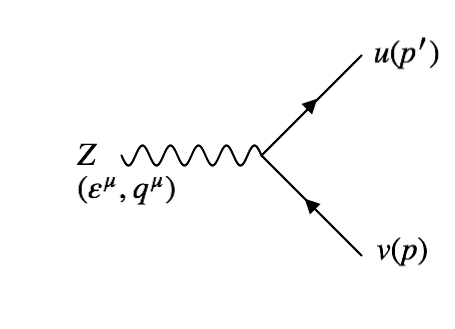
\includegraphics[width=0.6\textwidth]{images/web_feynman/image_57.png}
    \caption[Decay of $Z$ boson]{Decay of the $Z$ boson}
    \label{fig:ch13_ZToFF}
  \end{center}
\end{figure}

\[
  Z^0 \to f \quad \bar{f}
\]

where $f$ is any fermion, except the top quark.

\begin{eqnarray*}
  T_{fi} & = & \frac{g_W}{\cos\theta_W}\epsilon_{\mu}\bar{u}(p')\gamma^{\mu}\frac{1}{2}\left(c^f_V - c^f_A\gamma^5\right)v(p)\\
  \Rightarrow \Gamma & = & \frac{G_F M^3_Z}{6\sqrt{2}}\sqrt{1 - 4\eta}\Bigg[\left(1 - \eta\right)\Big[\left(c^f_V\right)^2 + \left(c^f_A\right)^2\Big] + 3\eta\Big[\left(c^f_V\right)^2 + \left(c^f_A\right)^2\Big]\Bigg] \\
  \textrm{where } \eta & = & \frac{m_f^2}{M^2_Z}
\end{eqnarray*}

Cross-section for $\e^+\e^- \stackrel{Z^0}{\to} f\bar{f}$:

\begin{figure}[!htb]
  \begin{center}
    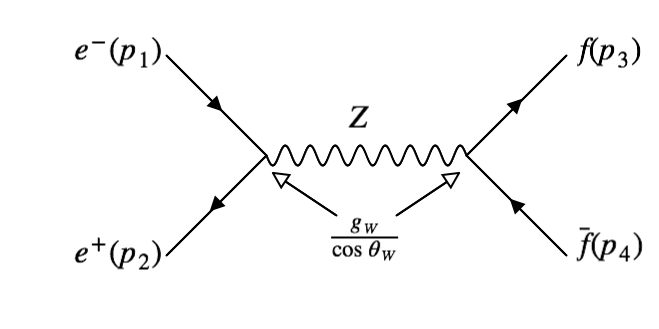
\includegraphics[width=0.8\textwidth]{images/web_feynman/image_58.png}
    \caption[Difermion production via the $Z$ boson]{Difermion production via the $e^+e^-\to Z\to f\bar{f}$ boson.}
    \label{fig:ch13_EEToZToFF}
  \end{center}
\end{figure}

\begin{eqnarray*}
  T_{fi} & = & \frac{g_W^2}{\cos\theta_W}\bar{v}(p_2)\gamma^{\mu}\left(\frac{c^{\e}_V - c^{\e}_A\gamma^5}{2}\right)u(p_1) \\
  & & \times \left(\frac{-g^{\mu\nu} + \frac{q^{\mu}q^{\nu}}{M^2_Z}}{s - M^2_Z - iM_Z\Gamma}\right)\bar{u}(p_4)\gamma_{\nu}\left(\frac{c^f_V - c^f_A\gamma^5}{2}\right)v(p_3)
\end{eqnarray*}

Then for unpolarised $\e^+\e^- \to \mu^+\mu^-$:

\[
  \frac{\mathrm{d}\sigma}{\mathrm{d}\Omega} = \frac{\alpha^2}{4s}\Big[A_0\left(1 + \cos^2\theta\right) + A_1\cos\theta\Big]
\]

where $\theta$ is the scattering angle.

$A_0$ and $A_1$ are functions of $c_V$ and $c_A$ and

\[
  \Gamma = \frac{\sqrt{2}G_FM_Z^2}{s - M_Z^2 - iM_Z\Gamma_Z}\left(\frac{s}{\e^2}\right)
\]

For lowest order QED $A_0 = 1$ and $A_1 = 0$ so the symmetric distribution is predicted.  The weak interaction introduces a forward-backward asymmetry.

Measurements at the $\e^+\e^-$ PETRA collider confirmed these interference effects at $\sqrt{s} = 34GeV$ of the virtual $Z/\gamma$ contributions by measuring the cross-section versus $\cos\theta$ and comparing with pure QED.

The cross-section at the $Z^0$ peak for $\e^+\e^- \to f\bar{f}$ is $\sim 30 nb$, however the resonance curve is strongly modified by radiative processes.

\begin{figure}[!htb]
  \begin{center}
    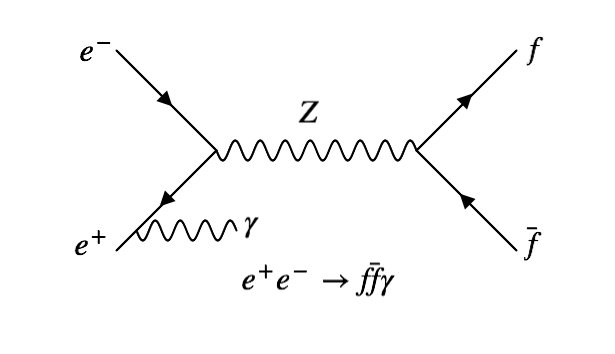
\includegraphics[width=0.8\textwidth]{images/web_feynman/image_59.png}
    \caption[Difermion production via the $Z$ boson with initial state radiation]{Difermion production via the $e^+e^-\to Z\to f\bar{f}\gamma$ boson with initial state radiation.}
    \label{fig:ch13_ZToFFGamma}
  \end{center}
\end{figure}


The matrix element of the above can be calculated.  This leads to a shift in the peak and a reduction of the peak cross-section.
